\chapter{Diseño del modelo}\label{chp-02}
\epigraph{I don't know where I'm going from here, but I promise it won't be boring.}{David Bowie}
\lettrine[lraise=-0.1, lines=2, loversize=0.2]{E}{ste} capítulo se centra en explicar el procedimiento seguido para la creación del modelo clasificador de audios.

Es importante destacar la gran cantidad de documentación existente además del gran apoyo que la comunidad ofrece en este campo en concreto.
Puede parecer un problema difícil de resolver, pero gracias a toda la información disponible y a la gran cantidad de herramientas que existen, ha sido posible crear un modelo capaz de ofrecer una funcionalidad básica.

En concreto, se destacan los sitios web \href{https://www.kaggle.com/}{Kaggle} y \href{https://huggingface.co/}{Hugging Face} como las principales fuentes de información y herramientas utilizadas.
Son dos plataformas directamente enfocadas al entrenamiento de modelos de \textit{Machine Learning} y \textit{Deep Learning}.
Ambas fomentan la colaboración entre usuarios y ofrecen una gran cantidad de recursos para la creación de modelos.

En concreto, se ha utilizado un dataset de \textit{Kaggle} para el entrenamiento del modelo y librerías específicos de Hugging Face para la creación del modelo en Python.


\section{Dataset}\label{seccion:dataset}
Como ha sido comentado en el \autoref{chp-01}, un problema que se enfrentó en el primer acercamiento a la problemática que este proyecto pretende resolver fue la falta de una base de datos que contuviera audios con las emociones específicas que se querían clasificar.
Al no haber impuesto restricciones, se ha optado por elegir un dataset ya existente.

La búsqueda de base de datos se ha realizado en \textit{Kaggle}.
La popularidad de esta plataforma no es injustificada, ya que cuenta con una gran cantidad de datasets de todo tipo.
En concreto, se han realizado búsquedas de datasets relacionados con audios clasificados por emociones.

En \textit{Kaggle} existen datasets oficiales creados por grandes organizaciones, y otros creados por usuarios de la plataforma.
La mayoría de los datasets son de libre acceso, por lo que tenemos la posibilidad de descargarlos y utilizarlos para nuestros propios proyectos.

En este caso, se ha optado por utilizar un dataset llamado \textit{Audio Emotions} compartido por el usuario \textit{Uldis Valainis}. \cite{Kaggle-dataset}
Este dataset es una recopilación de varios datasets similares creados por organizaciones diferentes, que contienen audios grabados por actores interpretando diferentes emociones.

La elección de este dataset se ha realizado por la gran cantidad de audios que contiene, y por tener un número variado de emociones.
Estas emociones son: \textit{neutral}, \textit{happy}, \textit{sad}, \textit{angry}, \textit{fearful}, \textit{disgust}, \textit{surprised}.

% """ insertar imagen de los audios del dataset """

\begin{figure}[htpb]
    \centering
    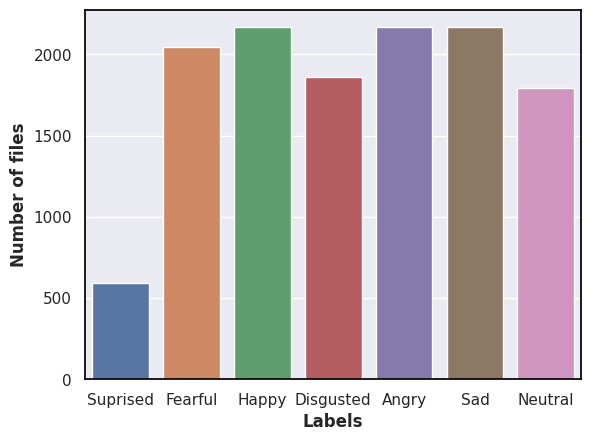
\includegraphics[width=0.8\textwidth]{cap2/images/dataset-bars.png}
    \caption{Número de audios del dataset}
    \label{fig:data-bars}
\end{figure}

% insert pie image
\begin{figure}[htpb]
    \centering
    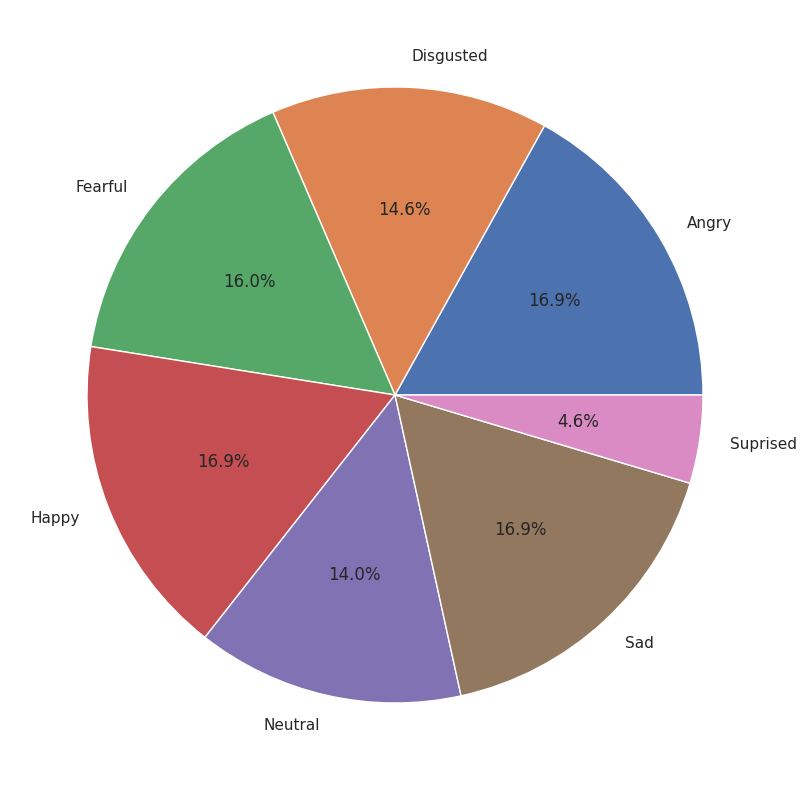
\includegraphics[width=0.8\textwidth]{cap2/images/dataset-pie.png}
    \caption{Porcentaje de audios del dataset}
    \label{fig:data-pie}
\end{figure}


El dataset contiene un total de 12.798 audios, con una duración de 3 segundos cada uno.

Echando un vistazo a la \autoref{fig:data-bars} y a la \autoref{fig:data-pie}, podemos observar una clara falta de balance en la clase \textit{surprised}, que contiene un número muy inferior de audios que el resto de clases.
Como no existen restricciones en cuanto a las clases que se quieren clasificar, se ha optado por eliminar esta clase del dataset, y quedarnos con las 6 clases restantes.
De este modo se consigue un dataset más equilibrado, lo cual influirá positivamente en el entrenamiento del modelo.

\begin{figure}[htpb]
    \centering
    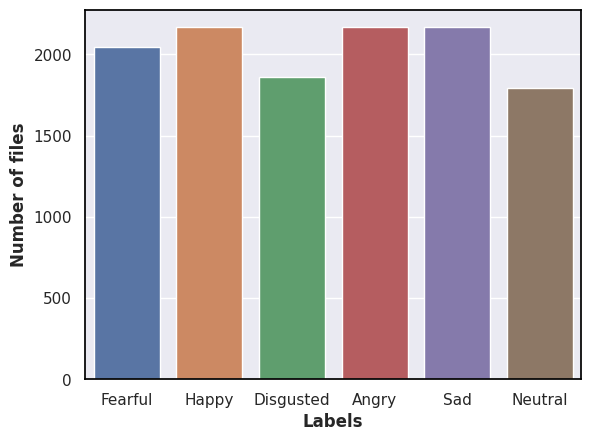
\includegraphics[width=0.8\textwidth]{cap2/images/dataset-bars-small.png}
    \caption{Número de audios del dataset reducido}
    \label{fig:data-bars-small}
\end{figure}

% insert pie image
\begin{figure}[htpb]
    \centering
    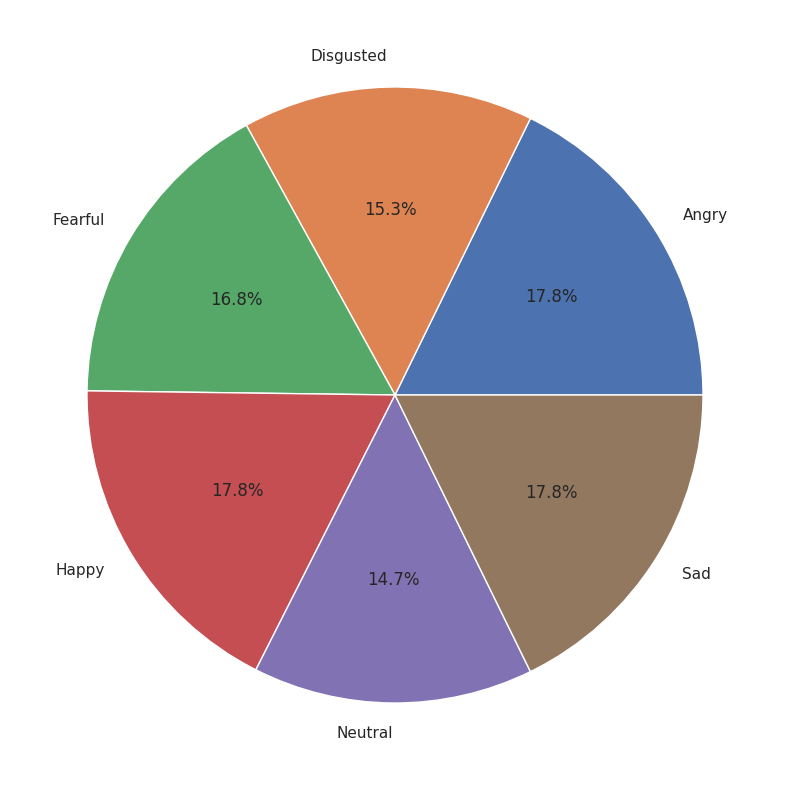
\includegraphics[width=0.8\textwidth]{cap2/images/dataset-pie-small.png}
    \caption{Porcentaje de audios del dataset reducido}
    \label{fig:data-pie-small}
\end{figure}

Esta versión del dataset cuenta con un total de 12.206 audios, con una duración de 3 segundos cada uno.

\section{Modelo}\label{seccion:modelo}
Una vez se ha seleccionado el dataset, se ha procedido a la creación del modelo.

\subsection{Estado del arte}\label{seccion:estado-del-arte}
Para poder enfocar un problema del que no se tiene conocimiento previo, es necesario realizar una investigación previa sobre el estado del arte, primero, para determinar si es posible resolver el problema, y segundo, para conocer las herramientas que existen para resolverlo.
En este caso, se ha realizado una investigación sobre las herramientas que existen para la clasificación de audios.

La solución parece estar ubicada en el campo de la \textit{Inteligencia Artificial}, y más concretamente en el campo del \textit{Deep Learning} debido a la dificultad de encontrar patrones en los audios.
Es importante saber clasificar nuestro problema dentro de un campo de la \textit{Inteligencia Artificial}, ya que existen diferentes herramientas para resolver problemas de diferentes campos.

Trabajos relacionados muestran un gran desempeño de la arquitectura conocida como \textbf{Transformers} en la clasificación de audios, ya que son capaces de capturar patrones en los audios que otras arquitecturas no son capaces de capturar.
Estos \textit{Transformers} son una arquitectura de \textit{Deep Learning} que se ha popularizado en los últimos años, y que ha demostrado un gran desempeño en la clasificación de textos y audios.
Por eso, son muy utilizados para tareas relacionadas con el campo del \textit{Natural Language Processing} (NLP), el campo del \textit{Speech Recognition} (SR), el campo del \textit{Speech Synthesis} (SS), y el campo del \textit{Emotion Recognition} (ER).

Desde que en 2017 salió a la luz el artículo \textit{Attention is all you need} \cite{vaswani2023attention}, en el que se presentaba la arquitectura \textit{Transformer}, se han realizado numerosos trabajos que han mostrado prometedores resultados en la clasificación de textos y audios. \cite{standfordCS224N} \cite{sullivan2022improving}

Sin embargo, su uso estaba reservado a grandes empresas con grandes recursos, ya que el entrenamiento de estos modelos requiere de una gran cantidad de datos y de una gran capacidad de cómputo.

Además de esto, la gran complejidad que presentaban hacía que su uso fuera muy complicado para usuarios con pocos conocimientos en el campo del \textit{Deep Learning}.
La aparición de librerías de un mayor nivel de abstracción ha acercado el uso de estas arquitecturas a usuarios con menos conocimientos.
Una de las librerías más utilizadas es \textit{Transformers}, desarrollada y mantenida por \textit{Hugging Face}, que ofrece una gran cantidad de herramientas para la carga de modelos pre-entrenados, realizar ajustes finos de estos modelos, procesar datos de entrada, etc.
Está pensado para poder ser usado por todo tipo de usuarios, desde usuarios con pocos conocimientos que quieran usar modelos pre-entrenados, usuarios con conocimientos avanzados que quieran realizar un ajuste fino de los modelos pre-entrenados, hasta investigadores que quieran crear sus propios modelos. \cite{transformers-docs}


\subsection{Elección del modelo}\label{seccion:eleccion-del-modelo}
Una vez se ha realizado una investigación sobre el estado del arte, se ha decidido utilizar un modelo pre-entrenado de los disponibles en la librería \textit{Transformers}.
Esta elección no es sencilla debido a la gran cantidad de opciones disponibles y la aparente similitud entre ellas.
Para poder elegir el modelo más adecuado, se ha realizado una búsqueda sobre cuáles son los modelos más utilizados en la clasificación de audios.

Tras investigar sobre los modelos más utilizados, se ha decidido utilizar el modelo \textit{Wav2Vec2} \cite{baevski2020wav2vec}
Este modelo ha sido creado por \textit{Facebook AI} específicamente para ser utilizado en tareas de los campos de \textit{Speech Recognition} (SR) y \textit{Audio Classification}.
Además, es un modelo popular entre usuarios de la librería \textit{Transformers}, incluso cuenta con ejemplos de uso en la documentación oficial de la librería.

Por estos motivos, se ha considerado más que apropiado para la resolución del problema que se plantea en este proyecto.

También ha sido empleado otro modelo bastante más grande, el modelo \textit{XLSR-Wav2Vec2} \cite{conneau2020unsupervised}.
Es una mejora del modelo "Wav2Vec2", que ha sido entrenado con una gran cantidad de datos de diferentes idiomas.
Este modelo ha sido utilizado para la clasificación de audios en diferentes idiomas, y se ha considerado interesante probarlo para la clasificación de audios en español.
La elección de este modelo se ha realizado con la finalidad de mejorar los resultados obtenidos con el modelo "Wav2Vec2", ya que es un modelo más versátil para la clasificación de audios en diferentes idiomas. \cite{greekEmotionRecognition}
Sin embargo, al ser más complejo requeriría una mayor capacidad de cómputo para su entrenamiento, además de un mejor ajuste de los parámetros.
Al no obtener mejores resultados que el modelo "Wav2Vec2", siendo más exigente computacionalmente, se ha decidido no utilizarlo en la solución final.


\section{Entrenamiento}\label{seccion:entrenamiento}
Una vez se ha seleccionado el modelo, se ha procedido a realizar el entrenamiento del mismo.

\subsection{Preparación del entrenamiento}\label{seccion:preparacion-del-entrenamiento}
Antes de comenzar el entrenamiento del modelo, es necesario realizar una serie de preparaciones previas.
La siguiente elección consiste en decidir qué librería de bajo nivel se va a utilizar para el entrenamiento del modelo.
\textit{Transformers} ofrece una documentación muy extensa con multitud de ejemplos en muchos campos, y dentro de estos ejemplos, podemos elegir entre \textit{PyTorch} y \textit{TensorFlow}, dos librerías de bajo nivel muy populares en el campo del \textit{Deep Learning}.

En principio no debe existir diferencia entre utilizar una u otra, ya que ambas librerías ofrecen las mismas funcionalidades.
Dependerá de la experiencia del usuario con una u otra, o de la preferencia del usuario.
En este caso, se ha optado por utilizar \textit{PyTorch}, ya que es una librería con la que se tiene algo más de experiencia, y además, es la librería que se utiliza en la documentación oficial de \textit{Transformers}.
Para un caso de uso en el que se requiera una mayor optimización de la solución, convendría estudiar más en profundidad las diferencias entre ambas librerías, y elegir la que mejor se adapte a las necesidades del usuario.

Una vez se ha elegido la librería de bajo nivel, se ha procedido a la preparación de los datos de entrada.
Los datos son en primer lugar descargos en una carpeta local.
Esta tarea es sencilla ya que \textit{Kaggle} permite cargar automáticamente los datos desde un script de Python.

Los datos no pueden ser introducidos directamente en la red neuronal, ya que esta espera recibir los datos en un formato específico.
Para esto, el modelo ofrece una herramienta que se encarga de procesar los datos de entrada y convertirlos en el formato que espera recibir la red neuronal.

El preprocesado de los datos, se basa en los siguientes pasos:
\begin{enumerate}
    \item Descarga de los datos desde \textit{Kaggle}.
    \item Descarte de la clase \textit{surprised}.
    \item Creación de un dataframe con los datos descargados.
    \item Conversión a objeto interpretable por la librería de Hugging Face.
    \item Mezcla de los datos y división en conjunto de entrenamiento y conjunto de test.
    \item Codificación de las etiquetas.
    \item Preparación del Feature Extractor de nuestro modelo.
    \item Procesado de los datos de entrada (frecuencia de muestreo y duración).
    
\end{enumerate}

\begin{lstlisting}[language=Python, caption=Preprocesado del dataset, label={code:download-data}]
from glob import glob
import pandas as pd
import datasets

# download dataset
import opendatasets as od
od.download("https://www.kaggle.com/datasets/uldisvalainis/audio-emotions")

df=pd.DataFrame(glob('audio-emotions/Emotions/*/*.wav'),columns=['paths'])

df['labels']=df.paths.apply(lambda x:x.split('/')[-2])

# drop rows where label is 'Surprised'
df=df[df.labels!='Suprised']


hf_data=datasets.Dataset.from_pandas(df)
hf_data=hf_data.class_encode_column("labels")#convert label to HF label class

hf_data=hf_data.train_test_split(train_size=0.8,seed=0)

# Create a dictionary that maps a label name to an integer and vice versa. The mapping will help the model recover the label name from the label number:
labels = hf_data['train'].features['labels'].names
label2id, id2label = dict(), dict()
for i, label in enumerate(labels):
    label2id[label] = str(i)
    id2label[str(i)] = label

#feature extractor
from transformers import AutoFeatureExtractor
model='facebook/wav2vec2-base-960h'
feature_extractor = AutoFeatureExtractor.from_pretrained(model)

#process the data such as fix sample rate
hf_data = hf_data.cast_column("paths", datasets.Audio(sampling_rate=16_000))

def preprocess_function(examples):
    audio_arrays = [x["array"] for x in examples["paths"]]
    inputs = feature_extractor(
        audio_arrays, sampling_rate=feature_extractor.sampling_rate, max_length=16000*2, truncation=True
    )
    return inputs


encoded_dataset = hf_data.map(preprocess_function, remove_columns=["paths"], batched=True)


\end{lstlisting}

% \medskip


\subsection{Entrenamiento del modelo}\label{seccion:entrenamiento-del-modelo}
Una vez se ha realizado el preprocesado de los datos, como se muestra en el \autoref{code:download-data}, podemos entrenar el modelo.

Debemos definir ahora la métrica que vamos a utilizar para evaluar el desempeño del modelo.
De este modo podremos calcular lo bien o mal que se comporta el modelo durante el entrenamiento, y así ir ajustando los pesos.

En este caso, se ha optado por utilizar la métrica \textit{accuracy}, que define la proporción de predicciones correctas realizadas por el modelo.
Para esta tarea, de nuevo, existe una librería de \textit{Hugging Face} que facilita la integración de esta métrica en el entrenamiento del modelo.

En este punto, podemos comenzar el entrenamiento del modelo.
La librería \textit{Transformers} permite guardar checkpoints del modelo durante el entrenamiento, de modo que podemos parar el entrenamiento en cualquier momento y continuar desde el último checkpoint guardado.
Una vez completado el entrenamiento, subiremos la mejor versión del modelo a la plataforma \textit{Hugging Face} para poder utilizarlo en producción.
De este modo nos aseguramos de que el modelo va a estar disponible en cualquier momento, y podemos compartirlo con otros usuarios, además de las ventajas que ofrecen los sistemas de control de versiones.

Los requisitos de seguridad de un proyecto real podrían requerir que el modelo no estuviera disponible públicamente, por lo que se debería buscar una alternativa para compartir el modelo con otros usuarios.
Como no es objetivo de este proyecto profundizar en este aspecto, se ha optado por aprovechar las ventajas de utilizar los servicios gratuitos que ofrece \textit{Hugging Face}.

El modelo desarrollado se encuentra disponible en la plataforma \textit{Hugging Face} guardado con el nombre de \textit{antonjaragon/emotions\_6\_classes\_small} donde se muestran los resultados, y podemos probar el modelo con audios de prueba.
Por otro lado, aunque no ha sido utilizado en este trabajo, también existe el modelo entrenado con el modelo \textit{XLSR-Wav2Vec2}, guardado con el nombre de \textit{antonjaragon/emotions\_6\_classes}.

En el \textbf{\href{https://huggingface.co/antonjaragon/emotions_6_classes_small}{repositorio}} se puede acceder a información más detallada sobre el entrenamiento del modelo, y se puede probar el modelo con audios de prueba.


\begin{lstlisting}[language=Python, caption=Entrenamiento del modelo, label={code:train-model}]
import evaluate
accuracy = evaluate.load("accuracy")

def compute_metrics(eval_preds):
    # metric = datasets.load_metric("accuracy")
    logits, labels = eval_preds
    predictions = np.argmax(logits, axis=1)
    return accuracy.compute(predictions=predictions, references=labels)

from transformers import AutoModelForAudioClassification, TrainingArguments, Trainer

num_labels = len(id2label)
model = AutoModelForAudioClassification.from_pretrained(model, num_labels=num_labels, label2id=label2id, id2label=id2label)

training_args = TrainingArguments(
    output_dir="./emotions",
    evaluation_strategy="epoch",
    save_strategy="epoch",
    fp16=True,
    learning_rate=3e-5,
    per_device_train_batch_size=32,
    gradient_accumulation_steps=4,
    per_device_eval_batch_size=32,
    num_train_epochs=10,
    warmup_ratio=0.1,
    logging_steps=10,
    load_best_model_at_end=True,
    metric_for_best_model="accuracy",
    push_to_hub=True,

)

trainer = Trainer(
    model=model,
    args=training_args,
    train_dataset=encoded_dataset['train'],
    eval_dataset=encoded_dataset["test"],
    tokenizer=feature_extractor,
    compute_metrics =compute_metrics,

)

trainer.train()

\end{lstlisting}


Las posibilidades de la librería \textit{Transformers} son muy amplias, y permiten realizar ajustes finos del modelo, como por ejemplo, la posibilidad de utilizar diferentes funciones de pérdidas, división de los datos en batches, diferentes métricas, etc.
Esto permite que el usuario pueda ajustar el modelo a sus necesidades, y pueda realizar un entrenamiento más eficiente.

En este caso, se ha optado por utilizar las opciones por defecto, e intentar mejorar resultados modificando algunos parámetros como el ratio de aprendizaje o el número de épocas de entrenamiento.
Al ser un procesamiento muy costoso, no se ha podido profundizar mucho en este aspecto, pero se ha conseguido un modelo que ofrece una funcionalidad básica.

Los resultados obtenidos por el mejor modelo tras el entrenamiento son los siguientes:
\begin{itemize}
    \item \textbf{Accuracy}: 0.7920
    \item \textbf{Loss}: 0.9106
\end{itemize} 


\section{Saturn Cloud}\label{seccion:saturn-cloud}
Para el entrenamiento del modelo, se ha hecho uso de los recursos gratuitos que ofrece la plataforma \textit{Saturn Cloud}.

El proceso de entrenamiento de un modelo de \textit{Deep Learning} implica un elevado coste computacional.
Las primeras pruebas se realizaron en un portátil personal con una tarjeta gráfica integrada.

Realizar entrenamientos pesados de varias horas de duración no es viable para un ordenador personal, ya que el desgaste sería muy elevado.
Por ello, se han buscado alternativas a probar en este proyecto en concreto.
Utilizar servicios de terceros para el entrenamiento de modelos puede no ser viable en muchos casos, debido a que necesitamos cargar los datos en la nube.
Esto puede ser un problema si los datos son sensibles, ya que no podemos garantizar la seguridad de los mismos.
Sin embargo, al estar utilizando un dataset público, no es un problema cargar los datos en el servidor de entrenamiento.

Además, el coste de utilizar estos servicios puede ser muy elevado, ya que el entrenamiento de un modelo puede durar varias horas, y el coste se calcula en función del tiempo de uso de los recursos.
Esta solución no sería la mejor para muchos escenarios, pero en este caso, se ha optado por utilizar los recursos gratuitos que ofrece la plataforma \textit{Saturn Cloud}.
La elección se debe a que es una de las pocas plataformas que ofrecen una instancia con GPU en el segmento gratuito.
Para nuevos usuarios, contamos con 150 horas de uso de una instancia con GPU, que es más que suficiente para realizar varios entrenamientos del modelo.

Este tipo de plataformas están directamente enfocadas al entrenamiento de modelos de \textit{Deep Learning}, por lo que ofrecen una gran cantidad de herramientas para facilitar el entrenamiento de modelos.
Existe multitud de imágenes pre-configuradas con las herramientas más utilizadas, y además, ofrecen la posibilidad de crear imágenes personalizadas con las herramientas que necesitemos.
En concreto, se han utilizado imágenes \textit{Debian} con \textit{PyTorch} pre-instalado.

\begin{figure}[htpb]
    \centering
    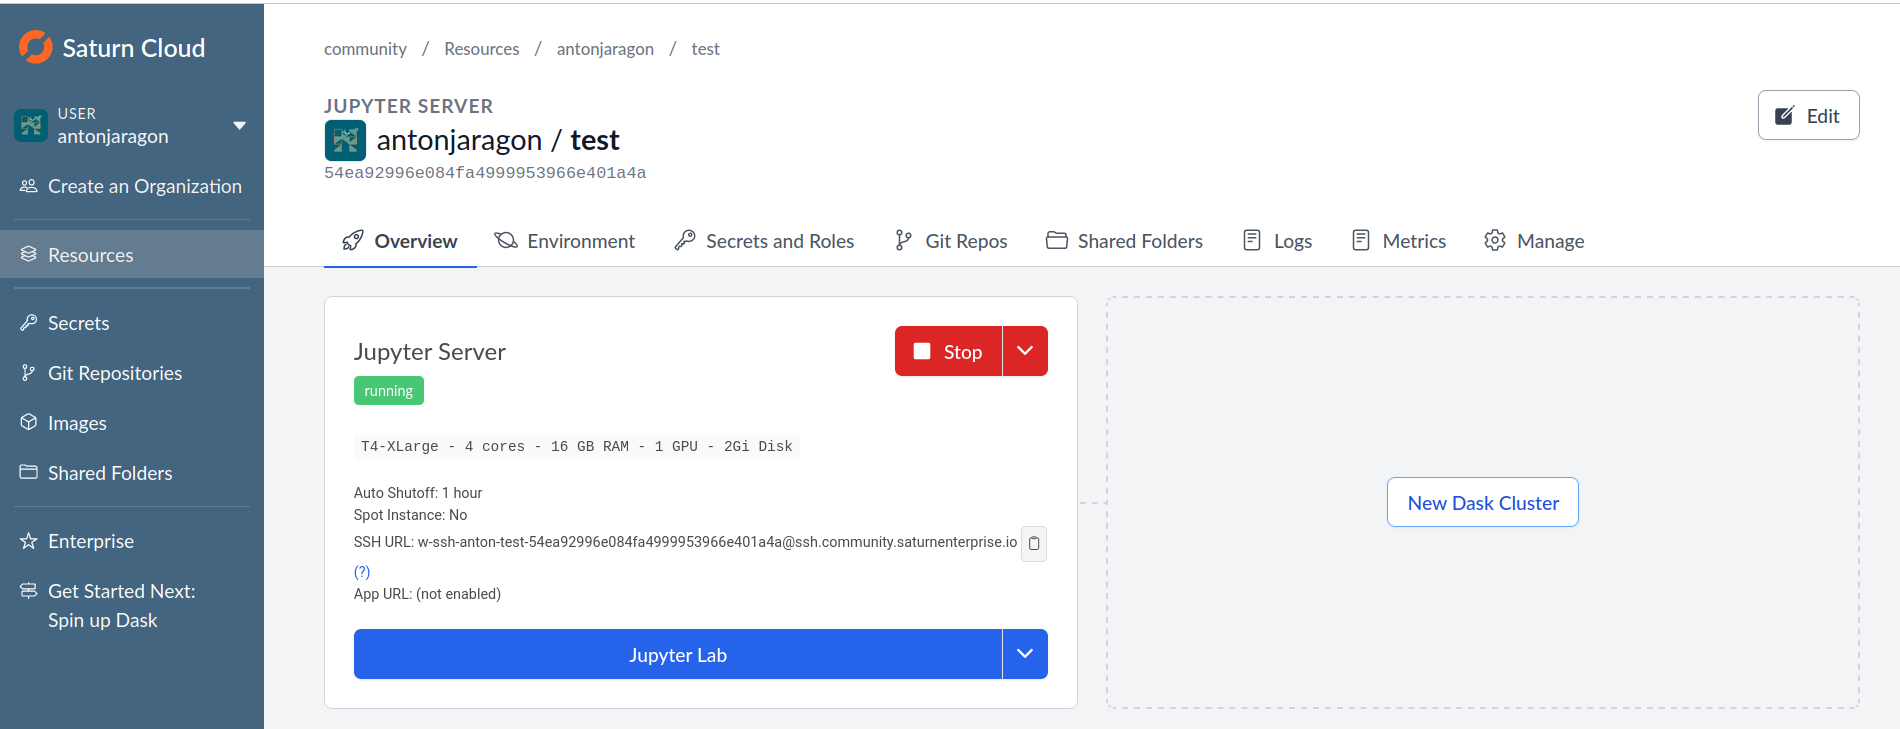
\includegraphics[width=0.8\textwidth]{cap2/images/saturn-cloud.png}
    \caption{Ejemplo de instancia activa con GPU en Saturn Cloud}
    \label{fig:saturn-cloud}
    
\end{figure}


\section{Evaluación del modelo}\label{seccion:evaluacion-del-modelo}
Conocemos el accuracy del modelo tras el entrenamiento, pero realmente no tenemos suficiente información para saber si el modelo es capaz de clasificar correctamente los audios.
Tampoco sabemos exactamente dónde podrían estar las debilidades del modelo, por lo que estaríamos a ciegas para intentar mejorar su desempeño.

Debemos extraer más información del modelo para poder evaluarlo correctamente.
Esta información ha sido obtenida mediante el cálculo de métricas de evaluación del modelo, y mediante la visualización de la matriz de confusión.

\subsection{Dataset de evaluación}\label{seccion:dataset-de-evaluacion}
Para poder evaluar el modelo, se ha utilizado un dataset diferente al utilizado para el entrenamiento.
El dataset elegido es el dataset \textit{AESDD} \cite{AESDD_1}\cite{AESDD_2}, que contiene audios grabados por actores interpretando diferentes emociones.

El idioma de los audios es el griego, cuenta con un total de 7.000 audios, y una duración de 3 a 10 segundos cada uno.
Están clasificados en las siguientes emociones: \textit{\textbf{anger}}, \textit{\textbf{disgust}}, \textit{\textbf{fear}}, \textit{\textbf{happiness}} y \textit{\textbf{sadness}}.

La elección de este dataset se debe principalmente a la similitud que presenta con el dataset utilizado para el entrenamiento.
Esto facilita la comparación de los resultados obtenidos con el modelo entrenado, y nos permite evaluar el desempeño del modelo en un escenario más realista.

Además, al ser un dataset de un idioma diferente, supone un reto mayor para el modelo, ya que no ha sido entrenado con audios en griego.
El modelo no es capaz de transcribir los audios, pero las emociones no son expresadas del mismo modo entre diferentes culturas.
Esta prueba nos ofrece una visión más realista de cómo se comportaría el modelo en un escenario real.

\subsection{Métricas de evaluación}\label{seccion:metricas-de-evaluacion}
Para calcular las métricas, se han realizado predicciones con el modelo sobre el dataset de evaluación.
Estas predicciones se han comparado con las etiquetas reales de los audios, y se han calculado las métricas de evaluación.

\subsubsection{Accuracy}\label{seccion:accuracy}
El \textit{accuracy} se define como la proporción de predicciones correctas realizadas por el modelo.
Es la métrica más utilizada para evaluar el desempeño de un modelo, ya que nos ofrece una visión general del desempeño del modelo.
También fue la métrica utilizada para evaluar el desempeño del modelo durante el entrenamiento.

% definicion de TP TN FP FN
Primero es necesario definir los términos \textit{True Positive}, \textit{True Negative}, \textit{False Positive} y \textit{False Negative}.
Son los resultados de una predicción, y se definen de la siguiente manera:
\begin{itemize}
    \item \textbf{True Positive (TP)}: El modelo predice correctamente la clase positiva.
    \item \textbf{True Negative (TN)}: El modelo predice correctamente la clase negativa.
    \item \textbf{False Positive (FP)}: El modelo predice incorrectamente la clase positiva.
    \item \textbf{False Negative (FN)}: El modelo predice incorrectamente la clase negativa.
\end{itemize}

El accuracy se calcula de la siguiente manera:

\begin{equation}
    Accuracy = \frac{TP + TN}{TP + TN + FP + FN} = 0.570
\end{equation}

Es un resultado bajo, pero hay que ponerlo en contexto.

El dataset fue sometido a un experimento en el que un grupo de personas clasificó los audios en las mismas clases que el modelo. \cite{AESDD_webpage}
El resultado obtenido fue un accuracy de 0.74, no muy lejos del resultado obtenido con el modelo.

De todos modos, es muy mejorable, pero no tenemos información sobre cómo mejorarlo.
Necesitamos más métricas.

\subsubsection{Precision}\label{seccion:precision}
La \textit{precision} se define como la proporción de predicciones positivas correctas entre el total de predicciones positivas realizadas por el modelo.
Nos informa de cuántas de las predicciones positivas son realmente positivas.
Es útil para detectar si los falsos positivos son un problema en nuestro modelo.

Se calcula de la siguiente manera:

\begin{equation}
    Precision = \frac{TP}{TP + FP}
\end{equation}

Como en este caso tenemos 5 clases, al cálculo de la predicción general se le aplica una media aritmética para obtener la precisión de cada clase.

% formula using average macro
\begin{equation}
    Precision = \frac{1}{n} \sum_{i=1}^{n} \frac{TP_i}{TP_i + FP_i} = 0.690
\end{equation}

En este caso, se ha calculado el valor medio de la suma de las precisiones de cada clase.
Hay diversos métodos para calcular la media, cada uno interpreta la precisión de una manera diferente.
Este método es el más directo, pero para obtener una visión más completa del desempeño del modelo, se deberían estudiar los resultados de cada clase por separado.

\subsubsection{Recall}\label{seccion:recall}
El \textit{recall} se define como la proporción de predicciones positivas correctas entre el total de predicciones positivas reales.
Se utiliza para determinar cuál es el mejor modelo en caso de tener un alto número de falsos negativos.

Se calcula de la siguiente manera:
\begin{equation}
    Recall = \frac{TP}{TP + FN}
\end{equation}

De nuevo, el método utilizado para calcular la media es el mismo que en el caso de la precisión.

\begin{equation}
    Recall = \frac{1}{n} \sum_{i=1}^{n} \frac{TP_i}{TP_i + FN_i} = 0.570
\end{equation}

\subsubsection{F1 Score}\label{seccion:f1-score}
El \textit{F1 Score} se define como la media armónica entre la precisión y el recall.
Es utilizado cuando se busca un equilibrio entre ambas métricas.

Se calcula de la siguiente manera:
\begin{equation}
    F1 Score = 2 * \frac{Precision * Recall}{Precision + Recall}
\end{equation}

De nuevo, el método utilizado para calcular la media es el mismo que en el caso de la precisión.

\begin{equation}
    F1 Score = \frac{1}{n} \sum_{i=1}^{n} 2 * \frac{Precision_i * Recall_i}{Precision_i + Recall_i} = 0.610
\end{equation}


% plot model metrics table

% Label: anger, F1 score: 0.617, Precision: 0.654, Recall: 0.583
% Label: disgust, F1 score: 0.033, Precision: 1.000, Recall: 0.017
% Label: fear, F1 score: 0.710, Precision: 0.598, Recall: 0.874
% Label: happiness, F1 score: 0.561, Precision: 0.435, Recall: 0.790
% Label: sadness, F1 score: 0.663, Precision: 0.763, Recall: 0.586

\begin{table}[htpb]
    \centering
    \begin{tabular}{|l|l|l|l|}
        \hline
        \textbf{Metric} & \textbf{Precision} & \textbf{Recall} & \textbf{F1 Score} \\ \hline
        \textbf{anger} & 0.654 & 0.583 & 0.617 \\ \hline
        \textbf{disgust} & 1.000 & 0.017 & 0.033 \\ \hline
        \textbf{fear} & 0.598 & 0.874 & 0.710 \\ \hline
        \textbf{happiness} & 0.435 & 0.790 & 0.561 \\ \hline
        \textbf{sadness} & 0.763 & 0.586 & 0.663 \\ \hline
    \end{tabular}
    \caption{Métricas de evaluación del modelo}
    \label{tab:model-metrics}
\end{table}


\subsubsection{Matriz de confusión}\label{seccion:matriz-de-confusion}
La matriz de confusión es una herramienta que nos permite visualizar los resultados de las predicciones realizadas por el modelo.
Muestra la cantidad de predicciones correctas e incorrectas realizadas por el modelo, organizadas por clase.

Nos permite obtener información sobre las relaciones entre las clases, de modo que podemos determinar cómo de bien identifica el modelo cada clase.
Es también una forma fácil de detectar si el modelo está confundiendo dos clases.

En nuestro caso, lo primero que salta a la vista al ver la \autoref{fig:confusion-matrix} es que el modelo no es capaz de identificar correctamente la clase \textit{disgust}.
Esto puede deberse a que quizás el etiquetado de audios es diferente entre el dataset de entrenamiento y el dataset de evaluación.

La matriz de confusión nos ha ayudado a descubrir este problema.
Mejorando el etiquetado de los dataset nos ayudaría a mejorar el accuracy.

Vemos también que la case \textit{fear} es la que mejor identifica el modelo, y la clase \textit{happiness} es la que peor identifica. 
Para mejorar este aspecto podríamos añadir más audios de la clase \textit{happiness} al dataset de entrenamiento. 



\begin{figure}
    \centering
    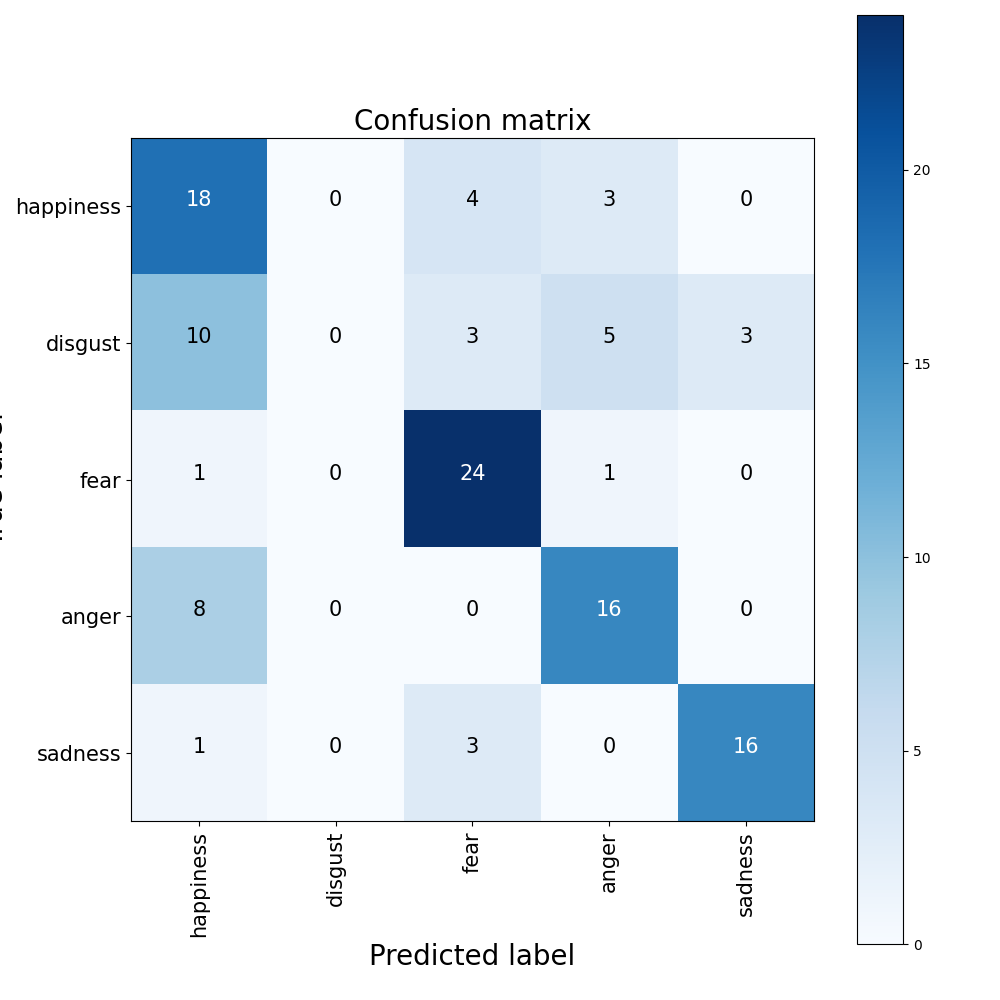
\includegraphics[width=0.8\textwidth]{cap2/images/confusion_matrix.png}
    \caption{Matriz de confusión del modelo}
    \label{fig:confusion-matrix}
\end{figure}


\begin{figure}
    \centering
    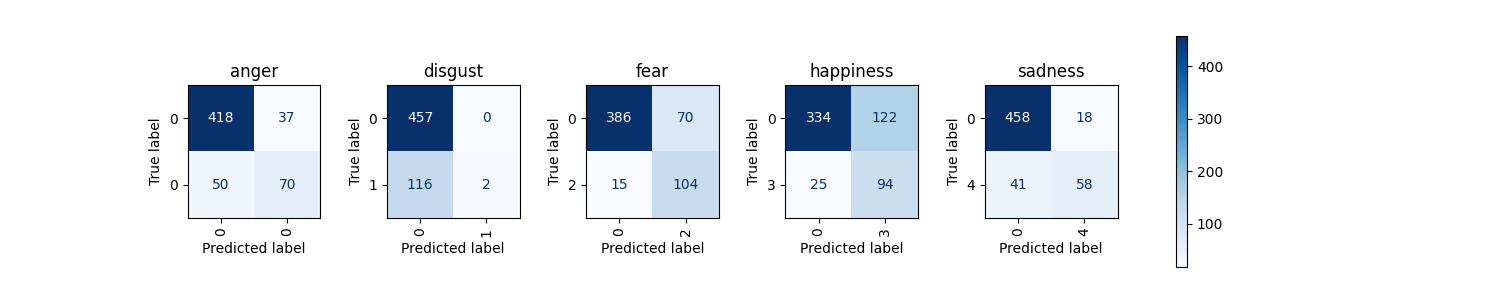
\includegraphics[width=0.8\textwidth]{cap2/images/multilabel_confusion_matrix.png}
    \caption{Matriz de confusión multi clase del modelo}
    \label{fig:confusion-matrix-multilabel}
\end{figure}


\begin{figure}
    \centering
    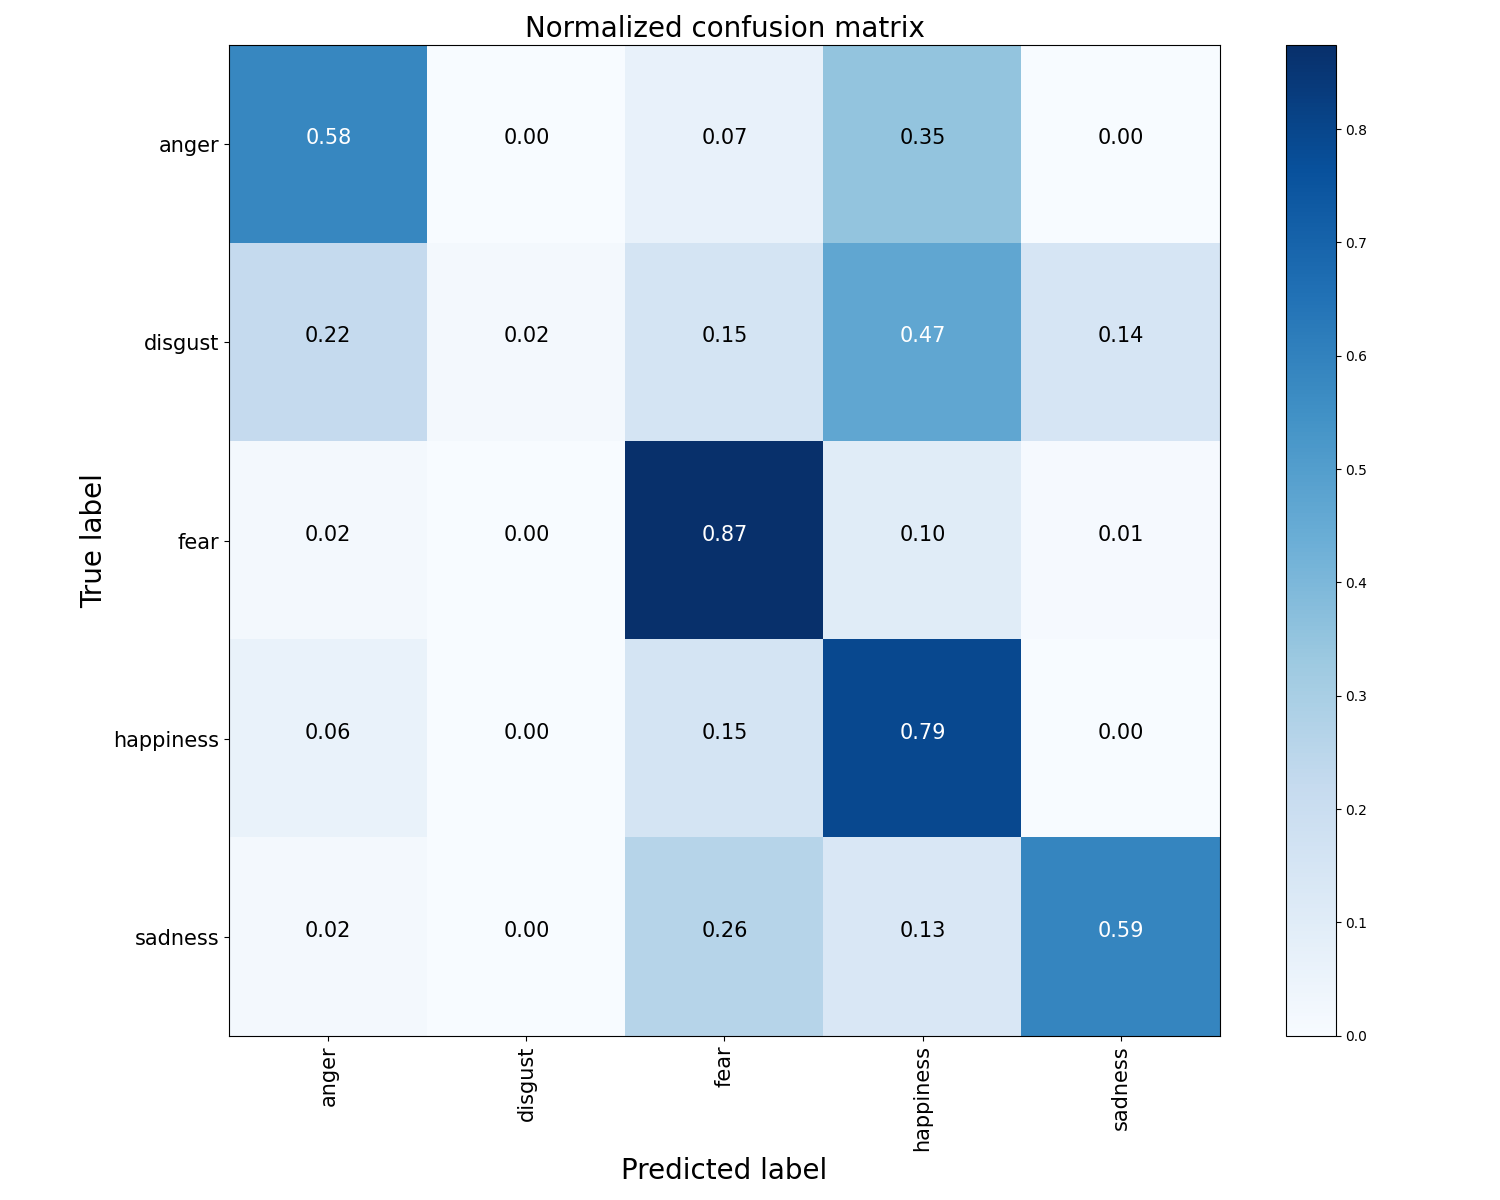
\includegraphics[width=0.8\textwidth]{cap2/images/normalized_confusion_matrix.png}
    \caption{Matriz de confusión normalizada del modelo}
    \label{fig:confusion-matrix-normalized}
\end{figure}




\endinput